\documentclass[letter,11pt,oneside,pdftex]{book}

\usepackage{verbatim}
\usepackage[spanish]{babel}
\usepackage[latin1]{inputenc}
\usepackage{lmodern}
\usepackage[T1]{fontenc}
\usepackage{textcomp}
\usepackage{float}
\renewcommand*\familydefault{\sfdefault}
\usepackage[pdftex]{graphicx}
\DeclareGraphicsExtensions{.pdf,.png,.jpg}

\newcommand{\ehmsof}{ehmSoft}
\newcommand{\softwareAbogadosMobile}{Procesos judiciales versi\'on m\'ovil~}
\newcommand{\blackberryos}[1]{BlackBerry\textsuperscript{\textregistered}~#1}
\newcommand{\blackberry}{BlackBerry\textsuperscript{\textregistered}~}
\newcommand{\insertImage}[3]{
\begin{figure}[H]
\begin{center}
\includegraphics[scale=0.4]{./CapturasDePantalla/#1.png}
\caption{#2}\label{fig:#3}
\end{center}
\end{figure}
}
\newcommand{\guardarVer}{Si al completar la edici\'on desea conservar los
cambios: lance el men\'u
\blackberry y seleccione guardar, de lo contrario presione la tecla
\emph{Escape} de su dispositivo.}

\usepackage[pdftex,colorlinks]{hyperref}
\hypersetup{linkcolor=black}

\title{}
\author{}
\date{}

\pdfinfo{%
  /Title    ()
  /Author   ()
  /Creator  ()
  /Producer ()
  /Subject  ()
  /Keywords ()
}

\begin{document}
%\maketitle
%\tableofcontents
\thispagestyle{empty}
\begin{figure}[c]
\begin{center}

\includegraphics[scale=0.3]{./CapturasDePantalla/logomanual.png}
\end{center}
\end{figure}
\frontmatter
\chapter{}
\blackberry y las marcas relacionadas pertenecientes a RIM, as\'i como las
im\'agenes y
s\'imbolos son propiedad exclusiva de Research In Motion Limited. RIM, Research
In
Motion,
BlackBerry, ``Always On, Always Connected'' y el s\'imbolo del ``sobre
en movimiento''
est\'an
registrados en la Oficina de Patentes y Marcas de EE.UU. y pueden estar
registradas o
pendientes de registro en otros pa\'ises.
Este documento se facilita ``tal cual'' y ehmSoftware S.A.S no asumen ning\'un
tipo
de
responsabilidad por posibles imprecisiones tipogr\'aficas, t\'ecnicas o de otro
tipo
en el
documento.
EN RELACI\'ON CON EL USO DE LA PRESENTE DOCUMENTACI\'ON, EN NING\'UN
CASO EHMSOFTWARE S.A.S NI SUS RESPECTIVOS DIRECTIVOS, RESPONSABLES,
EMPLEADOS O CONSULTORES ASUMIR\'AN RESPONSABILIDAD ALGUNA POR
CUALQUIER DA\~NO DIRECTO, ECON\'OMICO, COMERCIAL, ESPECIAL, RESULTANTE,
INCIDENTAL, EJEMPLAR O INDIRECTO, AUN CUANDO SE HAYA INFORMADO A
EHMSOFTWARE S.A.S DE MANERA EXPRESA SOBRE LA POSIBILIDAD DE PRODUCIRSE
TALES DA\~NOS, INCLUIDOS, SIN LIMITACIONES, DA\~NOS CAUSADOS POR P\'ERDIDA DE
BENEFICIOS O INGRESOS, P\'ERDIDA DE DATOS, RETRASOS, P\'ERDIDA DE GANANCIAS,
O BIEN LA IMPOSIBILIDAD DE ALCANZAR EL NIVEL DE AHORRO ESPERADO.
Este documento puede contener referencias a fuentes de informaci\'on, hardware o
software,
productos o servicios y/o sitios Web de terceros (de forma colectiva,
``informaci\'on de
terceros''). ehmSoftware S.A.S no controla ni es responsable de ning\'un tipo de
informaci\'on de
terceros, incluido, sin restricciones, el contenido, la exactitud, el
cumplimiento de copyright, la
compatibilidad, el rendimiento, la honradez, la legalidad, la decencia, los
v\'inculos o cualquier
otro aspecto de la informaci\'on de terceros.
\chapter{Introducci\'on}
\label{sec:intro}
\softwareAbogadosMobile es una aplicaci\'on para dispositivos \blackberry \\con
sistema operativo \blackberryos{5} o posterior, con esta aplicaci\'on usted puede llevar un
registro ordenado y de f\'acil acceso de sus procesos, incluyendo un listado de
demandantes, demandados, juzgados, actuaciones y dem\'as elementos importantes
en un proceso.
Adicionalmente podr\'a tener todas sus actuaciones presentes como citas en el
calendario de su dispositivo \blackberry con la posibilidad de una alarma como
recordatorio.

B\'asicamente \softwareAbogadosMobile es el complemento perfecto para su
trabajo, por su portabilidad y facilidad en el uso diario.
\tableofcontents
\mainmatter
\chapter{Primeros pasos}
\setcounter{page}{4}

\section{Obteniendo la aplicaci\'on}
Para obtener una copia de la \'ultima versi\'on de la aplicaci\'on ingrese con
su dispositivo \blackberry a la direcci\'on \emph{http://www.ehmsoft.com/ota},
all\'i confirma la descarga y despu\'es tendr\'a una versi\'on
totalmente funcional de la aplicaci\'on en su versi\'on m\'ovil.
\section{Ingresando por primera vez}
La primera vez que ingrese se le presentar\'a un mensaje con la licencia de la
aplicaci\'on, despu\'es de aceptarla ver\'a un di\'alogo en el que
introducir\'a la clave del producto que se le otorg\'o, cuando esta ha sido
validada estar\'a en una pantalla con fondo oscuro, esta es la pantalla inicial
de la aplicaci\'on.
\footnote{En caso de problemas con su clave de producto env\'ie un correo
electr\'onico a \mbox{soporte@ehmsoft.com}}


\section{Cosas que debe saber}
La aplicaci\'on cuenta con ciertos elementos que le ayudar\'an a tener una
mejor experiencia con la aplicaci\'on. A continuaci\'on se explicar\'an cuales
son dichos elementos:

\subsection{Buscador en cada listado}
Cuando aprenda sobre los listados
(P\'ag.\pageref{sec:consultandoLaInformacion}) podr\'a ver que todos ellos tienen
un buscador por defecto,
\footnote{Este puede ser desactivado en las preferencias
(P\'ag.\pageref{sec:busquedaPantallas})}
 con este podr\'a realizar b\'usquedas en tiempo real de cada campo que puede
contener cada elemento del listado. Para iniciar la b\'usqueda solamente tiene
que empezar a digitar la palabra que quiere buscar en el teclado de su
dispositivo \blackberry.
\subsection{Plantillas}
Son elementos \'utiles cuando usted desea crear procesos con
caracter\'isticas similares de forma r\'apida. Una plantilla contiene los mismos
campos de un proceso y en base a esta podr\'a crear procesos con esos campos
pre-ingresados.
\subsection{Campos personalizados}
En sus procesos y plantillas podr\'a agregar campos personalizados, estos son
\'utiles cuando usted desea agregar informaci\'on extra a un proceso. Por
ejemplo: Nombre del juez.
\subsection{Pantalla inicial}
La primera pantalla que ve al iniciar la aplicaci\'on tiene como funci\'on
informar las actuaciones que tienen vencimiento pr\'oximo en orden
cronol\'ogico.
\footnote{La cantidad mostrada puede ser modificada en las preferencias
(P\'ag. \ref{sec:actuacionesCriticas})}
Debe tener presente que una actuaci\'on pudo haberse vencido hace horas y aun
as\'i ser listada, esto se debe a que se muestran con respecto al d\'ia y no a
la hora de vencimiento, esto para evitar posibles p\'erdidas de citas.

En el listado puede observar si su cada actuaci\'on tiene una cita por medio de
los s\'imbolos de una campana para saber si tiene cita y un reloj indica si
tiene alarma.

Al situarse sobre una actuaci\'on podr\'a verla (editarla) desplegando el
men\'u \blackberry y seleccionando \emph{Ver actuaci\'on}. Tambi\'en podr\'a
ver el proceso asociado a una actuaci\'on desplegando el men\'u \blackberry y
seleccionando \emph{Ver proceso} (Fig. \ref{fig:pantallaInicialMenu}).

\begin{figure}[htb]
\begin{center}
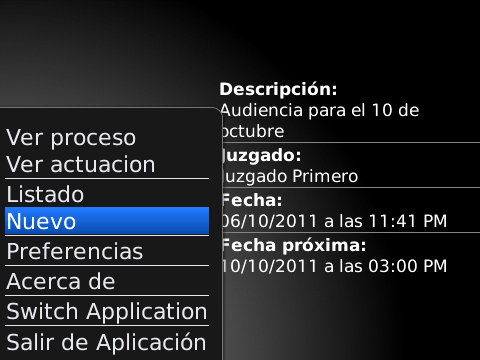
\includegraphics[scale=0.4]{./CapturasDePantalla/PantallaInicial/MenuPrincipal-Nuevo.png}
\caption{Men\'u en la pantalla inicial}\label{fig:pantallaInicialMenu}
\end{center}
\end{figure}
\chapter{Creando la informaci\'on}
\label{sec:creandoLaInformacion}
La creaci\'on de la informaci\'on se logra mediante pantallas de creaci\'on
independientes para cada elemento las cuales pueden ser accedidas por dos
m\'etodos principales:

\begin{description}
  \item[M\'etodo 1:]Por medio del men\'u \blackberry en la pantalla inicial,
  all\'i se selecciona \textit{Nuevo} (Fig.\ref{fig:nuevoPantallaInicial}) y
elige el elemento que desea crear en la lista
presentada (Fig.\ref{fig:listadoCrear})

\insertImage{PantallaInicial/MenuPrincipal-Nuevo}{Men\'u \emph{Nuevo} en la
pantalla inicial}{nuevoPantallaInicial}
\insertImage{Varios/ListaNuevo}{Nuevos elementos}{listadoCrear}
  \item[M\'etodo 2:]Por medio del men\'u \blackberry en la pantalla inicial,
  all\'i selecciona \textit{Listado} (Fig.\ref{fig:listadoPantallaInicial}) y
elige el listado del tipo que desea (Fig. \ref{fig:listadoListados}),
  despu\'es despliega el men\'u \blackberry y selecciona la opci\'on
\emph{Nuevo} (Fig. \ref{fig:nuevoElemento})
\insertImage{PantallaInicial/MenuPrincipal-Listado}{Men\'u \emph{Listado} en la
pantalla inicial}{listadoPantallaInicial}
\insertImage{Varios/ListaListado}{Listados de elementos}{listadoListados}
\insertImage{Listados/Demandante/Nuevo}{Nuevo elemento desde
listado}{nuevoElemento}
\end{description}

A continuaci\'on se describe el procedimiento para cada elemento usado por la
aplicaci\'on.

\section{Nuevo demandante}
\label{sec:nuevoDemandante}
Dir\'ijase a la pantalla inicial, despliegue el men\'u \blackberry y seleccione
\emph{Nuevo}, en este punto se le muestra un listado de los elementos posibles y
all\'i elija la opci\'on \emph{Demandante}.

Se presentar\'a una pantalla en la que podr\'a introducir toda la informaci\'on
que puede contener un demandante
\footnote{El campo Nombre se considera obligatorio y el campo Tel\'efono se
considera importante pero opcional},
cuando termine de ingresarla despliegue el men\'u \blackberry y seleccione
\emph{Guardar}.




\section{Nuevo demandado}
\label{sec:nuevoDemandado}
Dir\'ijase a la pantalla inicial, despliegue el men\'u \blackberry y seleccione
\emph{Nuevo}, en este punto se le muestra un listado de los elementos posibles y
all\'i elija la opci\'on \emph{Demandado}.

Se presentar\'a una pantalla en la que podr\'a introducir toda la informaci\'on
que puede contener un demandado
\footnote{El campo Nombre se considera obligatorio y el campo Tel\'efono se
considera importante pero opcional},
cuando termine de ingresarla despliegue el men\'u \blackberry y seleccione
\emph{Guardar}.
\section{Nuevo juzgado}
\label{sec:nuevoJuzgado}
Dir\'ijase a la pantalla inicial, despliegue el men\'u \blackberry y seleccione
\emph{Nuevo}, en este punto se le muestra un listado de los elementos posibles y
all\'i elija la opci\'on \emph{Juzgado}.

Se presentar\'a una pantalla en la que podr\'a introducir toda la informaci\'on
que puede contener un juzgado
\footnote{El campo Nombre se considera obligatorio y el campo Tel\'efono se
considera importante pero opcional},
cuando termine de ingresarla despliegue el men\'u \blackberry y seleccione
\emph{Guardar}.
\section{Nuevo campo personalizado}
\label{sec:nuevoCampo}
Dir\'ijase a la pantalla inicial, despliegue el men\'u \blackberry y seleccione
\emph{Nuevo}, en este punto se le muestra un listado de los elementos posibles y
all\'i elija la opci\'on \emph{Campo personalizado}.

Se presentar\'a una pantalla en la que podr\'a introducir el nombre del nuevo
campo personalizado
\footnote{El campo Nombre se considera obligatorio},
as\'i como tres
alternativas:
\begin{description}
\item[Obligatorio:]Es un campo de selecci\'on, que le permite determinar si el
campo que est\'a siendo creado, cuando se agregue a un proceso siempre
debe contener informaci\'on.
\item[Longitud m\'axima:]Es un campo para insertar n\'umeros, este tiene la
funci\'on de indicar que el campo que est\'a siendo creado, cuando se agregue a un proceso siempre debe tener informaci\'on de una longitud
m\'axima del valor introducido.
\footnote{Al ingresar 0 o dejarlo vac\'io indicar\'a que este par\'ametro
ser\'a ignorado}
\item[Longitud m\'inima:]Es un campo para insertar n\'umeros, este tiene la
funci\'on de indicar que el campo que est\'a siendo creado, cuando se agregue a un proceso siempre debe tener informaci\'on de una longitud
m\'inima del valor introducido.
\footnotemark[\value{footnote}]
\end{description}

Cuando termine de ingresar toda la informaci\'on despliegue el men\'u \blackberry y
seleccione \emph{Guardar}.
\section{Nueva categor\'ia}
\label{sec:nuevaCategoria}
Dir\'ijase a la pantalla inicial, despliegue el men\'u \blackberry y seleccione
\emph{Nuevo}, en este punto se le muestra un listado de los elementos posibles y
all\'i elija la opci\'on \emph{Categor\'ia}.

Se presentar\'a una pantalla en la que podr\'a introducir la descripci\'on de la
nueva categor\'ia.
\footnote{El campo Nombre se considera obligatorio},
cuando termine de ingresarla despliegue el men\'u \blackberry y seleccione
\emph{Guardar}.
\section{Nueva plantilla}
\label{sec:nuevaPlantilla}
Dir\'ijase a la pantalla inicial, despliegue el men\'u \blackberry y seleccione
\emph{Nuevo}, en este punto se le muestra un listado de los elementos posibles y
all\'i elija la opci\'on \emph{Plantilla}.

Se presentar\'a una pantalla en la que podr\'a introducir toda la informaci\'on
necesaria para su nueva plantilla. A continuaci\'on se describen las
caracter\'isticas de cada campo:
\begin{description}
\item[Nombre:]Es un campo de texto usado para diferenciar la plantilla, por lo
tanto se considera obligatorio ingresarlo.
\item[Demandante:]Es una etiqueta no editable que muestra el demandante
seleccionado, para cambiarlo solamente haga click sobre este
\footnote{Tambi\'en puede hacerlo desplegando el men\'u \blackberry y
seleccionando \emph{cambiar}}
e inmediatamente se
le mostrar\'a un listado con los demandantes existentes del cual podr\'a
seleccionar alguno.
\item[Demandado:]Es una etiqueta no editable que muestra el demandado
seleccionado, para cambiarlo solamente haga click sobre este
\footnotemark[\value{footnote}]
e inmediatamente.
se le mostrar\'a un listado con los demandados existentes del cual podr\'a
seleccionar alguno
\item[Juzgado:]Es una etiqueta no editable que muestra el juzgado
seleccionado, para cambiarlo solamente haga click sobre este
\footnotemark[\value{footnote}]
e inmediatamente
se le mostrar\'a un listado con los juzgados existentes del cual podr\'a
seleccionar alguno.
\item[Radicado:]Es un campo de texto en el que usted puede ingresar de manera
opcional el radicado que contendr\'a la plantilla.
\item[Radicado \'unico:]Es un campo de texto en el que usted puede ingresar de
manera opcional el radicado \'unico que contendr\'a la plantilla.
\item[Tipo:]Es un campo de texto en el que usted puede ingresar de manera
opcional el tipo que contendr\'a la plantilla.
\item[Estado:]Es un campo de texto en el que usted puede ingresar de manera
opcional el estado que contendr\'a la plantilla.
\item[Categor\'ia:]Es una etiqueta no editable que muestra la categor\'ia
a la que pertenece la plantilla actualmente, para cambiarla solamente haga click
sobre esta
\footnotemark[\value{footnote}]
e inmediatamente
se le mostrar\'a un listado con las categor\'ias existentes del cual podr\'a
seleccionar alguna.
\item[Prioridad:]Es un campo de selecci\'on, con este usted podr\'a asignarle
la prioridad a su nueva plantilla. \'Uselo haciendo click sobre este y
despu\'es seleccionando el valor deseado.
\item[Notas:]Es un campo de texto en el que usted puede ingresar de manera
opcional la nota que contendr\'a la plantilla.
\end{description}

\subsection{Agregando campos personalizados}
\label{sec:agregarCamposPlantilla}
Despliegue el men\'u \blackberry y seleccione \emph{Agregar campo personalizado}, se
presentar\'a un listado con los campos existentes, all\'i elija el campo
personalizado que desea a\~nadir al proceso.

\subsection{Modificando campos personalizados}
\label{sec:modificarCamposPlantilla}
Sit\'ue el cursor sobre el campo personalizado que desea modificar, y despliegue el
men\'u \blackberry, despu\'es seleccione \emph{Modificar},
se presentar\'a una pantalla en la que podr\'a modificar cada caracter\'istica
del campo personalizado. Esta pantalla se profundiza en la secci\'on
\ref{sec:verCampo} (Pag.\pageref{sec:verCampo}).

\subsection{Eliminando campos personalizado}
\label{sec:eliminarCamposPlantilla}
Sit\'ue el cursor sobre el campo personalizado que desea eliminar, y despliegue el
men\'u \blackberry, despu\'es seleccione \emph{Eliminar}.

Cuando termine de ingresar toda la informaci\'on despliegue el men\'u \blackberry y
seleccione \emph{Guardar}.
\section{Nueva actuaci\'on}
\label{sec:nuevaActuacion}
Dir\'ijase a la pantalla inicial, despliegue el men\'u \blackberry y seleccione
\emph{Nuevo}, en este punto se le muestra un listado de los elementos posibles y
all\'i elija la opci\'on \emph{Actuaci\'on}.

Se presentar\'a una pantalla en la que podr\'a introducir toda la informaci\'on
que puede contener una actuaci\'on. A continuaci\'on se describen las
caracter\'isticas de cada campo:

\begin{description}
\item[Juzgado:]Es una etiqueta no editable que muestra el juzgado
seleccionado, para cambiarlo solamente haga click sobre este
\footnote{Tambi\'en puede hacerlo desplegando el men\'u \blackberry y
seleccionando \emph{cambiar}}
e inmediatamente se le mostrar\'a un listado con los juzgados existentes del
cual podr\'a seleccionar alguno. Este campo se considera obligatorio.
\item[Fecha y fecha pr\'oxima:]Son campos de selecci\'on de fecha, para
modificarlos haga click sobre el elemento que desea editar (la fecha o la hora).
\item[Descripci\'on:]Es un campo de texto en el cual usted describir\'a la
nueva actuaci\'on. Este campo se considera obligatorio.
\end{description}

\subsection{Creando una cita}
\label{sec:crearCita}
Las actuaciones pueden contener citas, las cuales son agregadas al calendario
de su dispositivo \blackberry, estas tienen la posibilidad de tener una alarma
con la la anticipaci\'on que usted desee.

Despliegue el men\'u \blackberry y seleccione \emph{Agregar cita}, se mostrar\'a una
pantalla en la que podr\'a modificar la descripci\'on o la fecha pr\'oxima,
si selecciona el campo \emph{Alarma}, se activar\'a un campo adicional en el
que podr\'a especificar la anticipaci\'on y en el siguiente campo la duraci\'on
en minutos, horas o d\'ias. Cuando finalice presione \emph{Aceptar}
\footnote{La cita solamente ser\'a agregada o modificada en el calendario cuando
usted guarde la actuaci\'on}.

\subsection{Modificando una cita}
\label{sec:modificarCita}
Si la actuaci\'on ya contiene una cita pero desea modificarla, desplegando el
men\'u \blackberry encontrar\'a la opci\'on \emph{Modificar cita}, se
mostrar\'a una pantalla similar a la usada en la creaci\'on de una cita (Ver.
\ref{sec:crearCita}) en esta podr\'a modificar la informaci\'on de la cita
y seleccionando aceptar confirmar\'a los cambios
\footnotemark[\value{footnote}].

\subsection{Eliminando una cita}
\label{sec:eliminarCita}
Si la actuaci\'on ya contiene una cita pero desea eliminarla, desplegando el
men\'u \blackberry encontrar\'a la opci\'on \emph{Eliminar cita}, se mostrar\'a
un di\'alogo de confirmaci\'on y la cita ser\'a eliminada
\footnotemark[\value{footnote}].
\section{Nuevo Proceso}
\label{sec:nuevoProceso}
Dir\'ijase a la pantalla inicial, despliegue el men\'u \blackberry y seleccione
\emph{Nuevo}, en este punto se le muestra un listado de los elementos posibles y
all\'i elija la opci\'on \emph{Proceso}.

Se presentar\'a una pantalla en la que podr\'a introducir toda la informaci\'on
que puede contener un proceso A continuaci\'on se describen las
caracter\'isticas de cada campo:
\begin{description}
\item[Demandante:]Es una etiqueta no editable que muestra el demandante
seleccionado, para cambiarlo solamente haga click sobre este
\footnote{Tambi\'en puede hacerlo desplegando el men\'u \blackberry y
seleccionando \emph{cambiar}}
e inmediatamente se
le mostrar\'a un listado con los demandantes existentes del cual podr\'a
seleccionar alguno.
\item[Demandado:]Es una etiqueta no editable que muestra el demandado
seleccionado, para cambiarlo solamente haga click sobre este
\footnotemark[\value{footnote}]
e inmediatamente
se le mostrar\'a un listado con los demandados existentes del cual podr\'a
seleccionar alguno.
\item[Juzgado:]Es una etiqueta no editable que muestra el juzgado
seleccionado, para cambiarlo solamente haga click sobre este
\footnotemark[\value{footnote}]
e inmediatamente
se le mostrar\'a un listado con los juzgados existentes del cual podr\'a
seleccionar alguno.
\item[Radicado:]Es un campo de texto en el que usted puede ingresar de manera
opcional el radicado que contendr\'a el proceso.
\item[Radicado \'unico:]Es un campo de texto en el que usted puede ingresar de
manera opcional el radicado \'unico que contendr\'a el proceso.
\item[Tipo:]Es un campo de texto en el que usted puede ingresar de manera
opcional el tipo que contendr\'a el proceso.
\item[Estado:]Es un campo de texto en el que usted puede ingresar de manera
opcional el estado que contendr\'a el proceso.
\item[Categor\'ia:]Es una etiqueta no editable que muestra la categor\'ia
a la que pertenece el proceso actualmente, para cambiarla solamente haga click
sobre esta
\footnotemark[\value{footnote}]
e inmediatamente
se le mostrar\'a un listado con las categor\'ias existentes del cual podr\'a
seleccionar alguna.
\item[Prioridad:]Es un campo de selecci\'on, con este usted podr\'a asignarle
la prioridad a su nuevo proceso. \'Uselo haciendo click sobre este y
despu\'es seleccionando el valor deseado.
\item[Notas:]Es un campo de texto en el que usted puede ingresar de manera
opcional la nota que contendr\'a el proceso.
\end{description}

\subsection{Agregando campos personalizados}
\label{sec:agregarCamposProceso}
Despliegue el men\'u \blackberry y seleccione \emph{Agregar campo personalizado}, se
presentar\'a un listado con los campos existentes, all\'i elija el campo
personalizado que desea a\~nadir al proceso.

\subsection{Modificando campos personalizados}
\label{sec:modificarCamposProceso}
Sit\'ue el cursor sobre el campo personalizado que desea modificar, y despliegue el
men\'u \blackberry, despu\'es seleccione \emph{Modificar},
se presentar\'a una pantalla en la que podr\'a modificar cada caracter\'istica
del campo personalizado. Esta pantalla se profundiza en la secci\'on
\ref{sec:verCampo} (Pag.\pageref{sec:verCampo}).

\subsection{Eliminando campos personalizado}
\label{sec:eliminarCamposProceso}
Sit\'ue el cursor sobre el campo personalizado que desea eliminar, y despliegue el
men\'u \blackberry, despu\'es seleccione \emph{Eliminar}.

\subsection{Agregando actuaciones}
\label{sec:agregarActuacionesProceso}
Despliegue el men\'u \blackberry y seleccione \emph{Nueva actuaci\'on} y se
presentar\'a la pantalla para crear una nueva actuaci\'on (Ver.
\ref{sec:nuevaActuacion}).

\subsection{Ver actuaciones}
\label{sec:verActuacionesProceso}
Despliegue el men\'u \blackberry y seleccione \emph{Ver actuaciones}, se le
presentar\'a un listado con las actuaciones pertenecientes a este proceso y
haciendo click en cada una podr\'a ver la informaci\'on que contienen. (Ver.
\ref{sec:listadoActuaciones} Pag. \pageref{sec:listadoActuaciones})

\subsection{Eliminando actuaciones}
\label{sec:eliminarActuacionesProceso}
Despliegue el men\'u \blackberry y seleccione \emph{Ver actuaciones}, se le
presentar\'a un listado con las actuaciones pertenecientes a este proceso y
desplegando el men\'u \blackberry nuevamente selecciona la opci\'on
\emph{Eliminar}.

Cuando termine de ingresar toda la informaci\'on despliegue el men\'u \blackberry y
seleccione \emph{Guardar}.


\section{Proceso a partir de plantilla}
\label{sec:procesoPlantilla}

Dir\'ijase a la pantalla inicial, despliegue el men\'u \blackberry y seleccione
\emph{Nuevo}, en este punto se le muestra un listado de los elementos posibles y
all\'i elija la opci\'on \emph{Proceso a partir de plantilla}.

Se presentar\'a una pantalla con el listado de plantillas existentes y haciendo
click en una plantilla se desplegar\'a el dialogo de crear proceso (Ver.
\ref{sec:nuevoProceso}) con la informaci\'on de la plantilla ya incluída.



\chapter{Consultando la informaci\'on}
\label{sec:consultandoLaInformacion}
La consulta de la informaci\'on es posible realizarla por medio de dos
m\'etodos relacionados:

\begin{description}
  \item[M\'etodo 1:]Por medio de los \emph{listados} en los que se puede ver la
  colecci\'on de elementos del mismo tipo.
  Puede acceder a estas por medio del men\'u \blackberry en
  la pantalla inicial, all\'i se selecciona \textit{Listado} (Fig.
\ref{fig:listadoPantallaInicial}) y en la ventaja emergente elije el tipo de
  elemento que se  desea listar (Fig. \ref{fig:listadoListados})
\insertImage{PantallaInicial/MenuPrincipal-Listado}{Men\'u \emph{Listado} en la
pantalla inicial}{listadoPantallaInicial}
\insertImage{Varios/ListaListado}{Listados de elementos}{listadoListados}
  \item[M\'etodo 2:]Por medio de las \emph{Pantallas de edici\'on} o de
  visualizaci\'on, estas sirven para explorar cada elemento individual.
  Puede acceder a estas estando en un listado haciendo click en cualquier
  elemento  se lanzar\'a la pantalla de \emph{ver (editar)} (Fig.
\ref{fig:verProceso})
\insertImage{Ver/Proceso/Normal}{Pantalla de \emph{Ver}
proceso}{verProceso}

\end{description}

A continuaci\'on se describe el procedimiento para cada elemento usado por la
aplicaci\'on.

\section{Listado de actuaciones}
\label{sec:listadoActuaciones}
Dir\'ijase a la pantalla inicial, despliegue el men\'u \blackberry y seleccione
\emph{Listado}, en este punto se le muestra una lista de los elementos posibles
y all\'i elija la opci\'on \emph{Actuaci\'on}, se le presentar\'an sus procesos
de los cuales al seleccionar alguno se le mostrar\'a una pantalla
con sus actuaciones.

Estando en la pantalla podr\'a ver, eliminar y crear nuevas
actuaciones de la siguiente forma:

\begin{description}
\item[Ver y modificar actuaci\'on:]Haciendo click o desplegando el men\'u
\blackberry y seleccionando \emph{Ver}, se le presentar\'a la pantalla de
edici\'on que puede ver en la secci\'on \ref{sec:verActuacion} (P\'ag.
\pageref{sec:verActuacion}).
\item[Eliminar actuaci\'on:]Despliegue el men\'u \blackberry y seleccione
\emph{Eliminar}, confirme su acci\'on y la actuaci\'on ser\'a eliminada
definitivamente.
\item[Crear actuaci\'on:]Despliegue el men\'u \blackberry y seleccione \emph{Nuevo},
se le presentar\'a la pantalla vista en la secci\'on \ref{sec:nuevaActuacion}
(P\'ag. \pageref{sec:nuevaActuacion}).
\footnote{Tambi\'en como primer elemento de la lista se presenta una opci\'on
para crear un nuevo elemento}
\end{description}


\section{Ver actuaci\'on}
\label{sec:verActuacion}
Esta pantalla sirve para ver todo el contenido de una actuaci\'on as\'i como
su cita asociada (en caso de contener alguna). Adem\'as podr\'a editar los
elementos que desee, incluyendo la cita. Para acceder a esta despliegue el
\emph{Listado de actuaciones} (Ver \ref{sec:listadoActuaciones}) y haga click
en la actuaci\'on que desea ver.

Estando en esta pantalla podr\'a visualizar o editar la informaci\'on as\'i:

\begin{description}
\item[Editar campos individuales:]Para editar cualquier campo que contenga
informaci\'on despliegue el men\'u \blackberry y seleccione \emph{Editar},
inmediatamente el campo
cambiar\'a de estado podr\'a y ser modificado.
\item[Editar todo:]despliegue el men\'u \blackberry y seleccione \emph{Editar todo},
de esta forma todos los campos pasar\'an a ser editables.
\item[Eliminar actuaci\'on:]Para eliminar la actuaci\'on que est\'a viendo
actualmente despliegue el men\'u \blackberry y seleccione \emph{Eliminar}, al
confirmar ser\'a eliminada definitivamente.
\end{description}

\guardarVer

\subsection{Creando una cita}
\label{sec:crearCita}
Las actuaciones pueden contener citas, las cuales son agregadas al calendario
de su dispositivo \blackberry, estas tienen la posibilidad de tener una alarma
con la la anticipaci\'on que usted desee.

Despliegue el men\'u \blackberry y seleccione \emph{Agregar cita}, se mostrar\'a una
pantalla en la que podr\'a modificar la descripci\'on o la fecha pr\'oxima,
si selecciona el campo \emph{Alarma}, se activar\'a un campo adicional en el
que podr\'a especificar la anticipaci\'on y en el siguiente campo la duraci\'on
en Minutos, hora o d\'ias. Cuando finalice presione \emph{Aceptar}
\footnote{La cita solamente ser\'a agregada o modificada en el calendario cuando
usted guarde la actuaci\'on}.

\subsection{Modificando una cita}
\label{sec:modificarCita}
Si la actuaci\'on ya contiene una cita pero desea modificarla, desplegando el
men\'u \blackberry encontrar\'a la opci\'on \emph{Modificar cita}, se
mostrar\'a una pantalla similar a la usada en la creaci\'on de una cita (Ver.
\ref{sec:crearCita}) en esta podr\'a modificar la informaci\'on de la cita
y seleccionando aceptar confirmar\'a los cambios
\footnotemark[\value{footnote}].

\subsection{Eliminando una cita}
\label{sec:eliminarCita}
Si la actuaci\'on ya contiene una cita pero desea eliminarla, desplegando el
men\'u \blackberry encontrar\'a la opci\'on \emph{Eliminar cita}, se mostrar\'a
un di\'alogo de confirmaci\'on y la cita ser\'a eliminada
\footnotemark[\value{footnote}].
\section{Listado de categor\'ias}
\label{sec:listadoCategorias}
Dir\'ijase a la pantalla inicial, despliegue el men\'u \blackberry y seleccione
\emph{Listado}, en este punto se le muestra una lista de los elementos posibles
y all\'i elija la opci\'on \emph{Categor\'ia}, se le mostrar\'a una pantalla
con sus categor\'ias.

Estando en la pantalla podr\'a ver, eliminar y crear nuevas
categor\'ias de la siguiente forma:

\begin{description}
\item[Ver y modificar categor\'ia:]Haciendo click o desplegando el men\'u
\blackberry y seleccionando \emph{Ver}, se le presentar\'a la pantalla de
edici\'on que puede ver en la secci\'on \ref{sec:verCategoria} (P\'ag.
\pageref{sec:verCategoria}).
\item[Eliminar categor\'ia:]Despliegue el men\'u \blackberry y seleccione
\emph{Eliminar}, confirme su acci\'on y la categor\'ia ser\'a eliminada
definitivamente.
\item[Crear categor\'ia:]Despliegue el men\'u \blackberry y seleccione \emph{Nuevo},
se le presentar\'a la pantalla vista en la secci\'on \ref{sec:nuevaCategoria}
(P\'ag. \pageref{sec:nuevaCategoria}).
\footnote{Tambi\'en como primer elemento de la lista se presenta una opci\'on
para crear un nuevo elemento}
\end{description}


\section{Ver categor\'ia}
\label{sec:verCategoria}
Esta pantalla sirve para ver y modificar la descripci\'on de la categor\'ia.
Para acceder a esta despliegue el \emph{Listado de categor\'ias}
(Ver \ref{sec:listadoCategorias}) y haga click en la categor\'ia que desea ver.

Estando en esta pantalla podr\'a visualizar o editar la informaci\'on as\'i:

\begin{description}
\item[Editar:]Para editar la descripci\'on despliegue el men\'u \blackberry
y seleccione \emph{Editar}, inmediatamente el campo cambiar\'a de estado
y podr\'a ser modificado.
\item[Eliminar categor\'ia:]Para eliminar la categor\'ia que esta viendo
actualmente despliegue el men\'u \blackberry y seleccione \emph{Eliminar}, al
confirmar la categor\'ia ser\'a eliminada definitivamente.
\end{description}

\guardarVer
\section{Listado de campos personalizados}
\label{sec:listadoCampos}
Dir\'ijase a la pantalla inicial, despliegue el men\'u \blackberry y seleccione
\emph{Listado}, en este punto se le muestra una lista de los elementos posibles
y all\'i elija la opci\'on \emph{Campo personalizado}, se le mostrar\'a una
pantalla con sus campos personalizados.

Estando en la pantalla podr\'a ver, eliminar y crear nuevos campos
personalizados de la siguiente forma:

\begin{description}
\item[Ver y modificar campo personalizado:]Haciendo click o desplegando el men\'u
\blackberry y seleccionando \emph{Ver}, se le presentar\'a la pantalla de
edici\'on que puede ver en la secci\'on \ref{sec:verCampo} (P\'ag.
\pageref{sec:verCampo}).
\item[Eliminar campo personalizado:]Despliegue el men\'u \blackberry y seleccione
\emph{Eliminar}, confirme su acci\'on y el campo personalizado ser\'a eliminado
definitivamente.
\item[Crear campo personalizado:]Despliegue el men\'u \blackberry y seleccione
\emph{Nuevo}, se le presentar\'a la pantalla vista en la
secci\'on \ref{sec:nuevoCampo}
(P\'ag. \pageref{sec:nuevoCampo}).
\footnote{Tambi\'en como primer elemento de la lista se presenta una opci\'on
para crear un nuevo elemento}
\end{description}

\section{Ver campo personalizado}
\label{sec:verCampo}
Esta pantalla sirve para ver todo el contenido de un campo personalizado y
podr\'a editar los elementos que desee. Para acceder a esta
despliegue el \emph{Listado de campos personalizados}
(Ver \ref{sec:listadoCampos}) y haga click en el campo personalizado que desea
ver.

Estando en esta pantalla podr\'a visualizar o editar la informaci\'on as\'i:

\begin{description}
\item[Editar campos individuales:]Para editar cualquier campo que contenga
informaci\'on despliegue el men\'u \blackberry y seleccione \emph{Editar},
inmediatamente el campo
cambiar\'a de estado podr\'a y ser modificado.
\item[Editar todo:]despliegue el men\'u \blackberry y seleccione \emph{Editar todo},
de esta forma todos los campos pasar\'an a ser editables.
\item[Eliminar campo personalizado:]Para eliminar el campo personalizado que
est\'a viendo actualmente despliegue el men\'u \blackberry y
seleccione \emph{Eliminar}, al confirmar, el campo personalizado ser\'a
eliminado definitivamente.
\end{description}
\guardarVer
\section{Listado de demandantes}
\label{sec:listadoDemandantes}
Dir\'ijase a la pantalla inicial, despliegue el men\'u \blackberry y seleccione
\emph{Listado}, en este punto se le muestra una lista de los elementos posibles
y all\'i elija la opci\'on \emph{Demandantes}, se le mostrar\'a una
pantalla con demandantes.

Estando en la pantalla podr\'a ver, eliminar y crear nuevos demandantes de la
siguiente forma:

\begin{description}
\item[Ver y modificar demandante:]Haciendo click o desplegando el men\'u
\blackberry y seleccionando \emph{Ver}, se le presentar\'a la pantalla de
edici\'on que puede ver en la secci\'on \ref{sec:verDemandante} (P\'ag.
\pageref{sec:verDemandante}).
\item[Eliminar demandante:]Despliegue el men\'u \blackberry y seleccione
\emph{Eliminar}, confirme su acci\'on y el demandante ser\'a eliminado
definitivamente.
\item[Crear demandante:]Despliegue el men\'u \blackberry y seleccione
\emph{Nuevo}, se le presentar\'a la pantalla vista en la
secci\'on \ref{sec:nuevoDemandante}
(P\'ag. \pageref{sec:nuevoDemandante}).
\footnote{Tambi\'en como primer elemento de la lista se presenta una opci\'on
para crear un nuevo elemento}
\end{description}

\section{Ver demandante}
\label{sec:verDemandante}
Esta pantalla sirve para ver todo el contenido de un demandante y
podr\'a editar los elementos que desee. Para acceder a esta
despliegue el \emph{Listado de demandantes}
(Ver \ref{sec:listadoDemandantes}) y haga click en el demandante que
desea ver.

Estando en esta pantalla podr\'a visualizar o editar la informaci\'on as\'i:

\begin{description}
\item[Editar campos individuales:]Para editar cualquier campo que contenga
informaci\'on despliegue el men\'u \blackberry y seleccione \emph{Editar},
inmediatamente el campo
cambiar\'a de estado podr\'a y ser modificado.
\item[Editar todo:]despliegue el men\'u \blackberry y seleccione \emph{Editar todo},
de esta forma todos los campos pasar\'an a ser editables.
\item[Eliminar demandante:]Para eliminar el demandante que
est\'a viendo actualmente despliegue el men\'u \blackberry y
seleccione \emph{Eliminar}, al confirmar, el demandante ser\'a
eliminado definitivamente.
\end{description}

\guardarVer
\section{Listado de demandados}
\label{sec:listadoDemandados}
Dir\'ijase a la pantalla inicial, despliegue el men\'u \blackberry y seleccione
\emph{Listado}, en este punto se le muestra una lista de los elementos posibles
y all\'i elija la opci\'on \emph{Demandados}, se le mostrar\'a una
pantalla con demandados.

Estando en la pantalla podr\'a ver, eliminar y crear nuevos demandados de la
siguiente forma:

\begin{description}
\item[Ver y modificar demandado:]Haciendo click o desplegando el men\'u
\blackberry y seleccionando \emph{Ver}, se le presentar\'a la pantalla de
edici\'on que puede ver en la secci\'on \ref{sec:verDemandado} (P\'ag.
\pageref{sec:verDemandado}).
\item[Eliminar demandado:]Despliegue el men\'u \blackberry y seleccione
\emph{Eliminar}, confirme su acci\'on y el demandado ser\'a eliminado
definitivamente.
\item[Crear demandado:]Despliegue el men\'u \blackberry y seleccione
\emph{Nuevo}, se le presentar\'a la pantalla vista en la
secci\'on \ref{sec:nuevoDemandado}
(P\'ag. \pageref{sec:nuevoDemandado}).
\footnote{Tambi\'en como primer elemento de la lista se presenta una opci\'on
para crear un nuevo elemento}
\end{description}

\section{Ver demandado}
\label{sec:verDemandado}
Esta pantalla sirve para ver todo el contenido de un demandado y
podr\'a editar los elementos que desee. Para acceder a esta
despliegue el \emph{Listado de demandados}
(Ver \ref{sec:listadoDemandados}) y haga click en el demandado que
desea ver.

Estando en esta pantalla podr\'a visualizar o editar la informaci\'on as\'i:

\begin{description}
\item[Editar campos individuales:]Para editar cualquier campo que contenga
informaci\'on despliegue el men\'u \blackberry y seleccione \emph{Editar},
inmediatamente el campo
cambiar\'a de estado podr\'a y ser modificado.
\item[Editar todo:]despliegue el men\'u \blackberry y seleccione \emph{Editar todo},
de esta forma todos los campos pasar\'an a ser editables.
\item[Eliminar demandado:]Para eliminar el demandado que
est\'a viendo actualmente despliegue el men\'u \blackberry y
seleccione \emph{Eliminar}, al confirmar, el demandado ser\'a
eliminado definitivamente.
\end{description}

\guardarVer
\section{Listado de juzgados}
\label{sec:listadoJuzgados}
Dir\'ijase a la pantalla inicial, despliegue el men\'u \blackberry y seleccione
\emph{Listado}, en este punto se le muestra una lista de los elementos posibles
y all\'i elija la opci\'on \emph{Juzgados}, se le mostrar\'a una
pantalla con sus juzgados.

Estando en la pantalla podr\'a ver, eliminar y crear nuevos juzgados de la
siguiente forma:

\begin{description}
\item[Ver y modificar juzgado:]Haciendo click o desplegando el men\'u
\blackberry y seleccionando \emph{Ver}, se le presentar\'a la pantalla de
edici\'on que puede ver en la secci\'on \ref{sec:verJuzgado} (P\'ag.
\pageref{sec:verJuzgado}).
\item[Eliminar juzgado:]Despliegue el men\'u \blackberry y seleccione
\emph{Eliminar}, confirme su acci\'on y el juzgado ser\'a eliminado
definitivamente.
\item[Crear juzgado:]Despliegue el men\'u \blackberry y seleccione
\emph{Nuevo}, se le presentar\'a la pantalla vista en la
secci\'on \ref{sec:nuevoJuzgado}
(P\'ag. \pageref{sec:nuevoJuzgado}).
\footnote{Tambi\'en como primer elemento de la lista se presenta una opci\'on
para crear un nuevo elemento}
\end{description}

\section{Ver juzgado}
\label{sec:verJuzgado}
Esta pantalla sirve para ver todo el contenido de un juzgado y
podr\'a editar los elementos que desee. Para acceder a esta
despliegue el \emph{Listado de juzgados}
(Ver \ref{sec:listadoJuzgados}) y haga click en el juzgados que
desea ver.

Estando en esta pantalla podr\'a visualizar o editar la informaci\'on as\'i:

\begin{description}
\item[Editar campos individuales:]Para editar cualquier campo que contenga
informaci\'on despliegue el men\'u \blackberry y seleccione \emph{Editar},
inmediatamente el campo
cambiar\'a de estado podr\'a y ser modificado.
\item[Editar todo:]despliegue el men\'u \blackberry y seleccione \emph{Editar todo},
de esta forma todos los campos pasar\'an a ser editables.
\item[Eliminar juzgado:]Para eliminar el juzgado que
est\'a viendo actualmente despliegue el men\'u \blackberry y
seleccione \emph{Eliminar}, al confirmar ser\'a eliminado definitivamente.
\end{description}

\guardarVer
\section{Listado de procesos}
\label{sec:listadoProcesos}
Dir\'ijase a la pantalla inicial, despliegue el men\'u \blackberry y seleccione
\emph{Listado}, en este punto se le muestra una lista de los elementos posibles
y all\'i elija la opci\'on \emph{Procesos}, se le mostrar\'a una
pantalla con sus procesos.

Estando en la pantalla podr\'a ver, eliminar y crear nuevos procesos de la
siguiente forma:

\begin{description}
\item[Ver y modificar proceso:]Haciendo click o desplegando el men\'u
\blackberry y seleccionando \emph{Ver}, se le presentar\'a la pantalla de
edici\'on que puede ver en la secci\'on \ref{sec:verProceso} (P\'ag.
\pageref{sec:verProceso}).
\item[Eliminar proceso:]Despliegue el men\'u \blackberry y seleccione
\emph{Eliminar}, confirme su acci\'on y el proceso ser\'a eliminado
definitivamente.
\item[Crear proceso:]Despliegue el men\'u \blackberry y seleccione
\emph{Nuevo}, se le presentar\'a la pantalla vista en la
secci\'on \ref{sec:nuevoProceso} (P\'ag. \pageref{sec:nuevoJuzgado}).
\footnote{Tambi\'en como primer elemento de la lista se presenta una opci\'on
para crear un nuevo elemento}
\end{description}

\section{Ver proceso}
\label{sec:verProceso}
Esta pantalla sirve para ver todo el contenido de un proceso as\'i como sus
actuaciones asociadas, adem\'as podr\'a editar los elementos que desee. Para
acceder a esta despliegue el \emph{Listado de juzgados} (Ver
\ref{sec:listadoProcesos}) y haga click en el proceso que desea ver.

A continuaci\'on se describen las caracter\'isticas de cada campo:

\begin{description}
\item[Demandante:]Es una etiqueta no editable que muestra el demandante
seleccionado, para cambiarlo solamente haga click sobre este
\footnote{Tambi\'en puede hacerlo desplegando el men\'u \blackberry y
seleccionando \emph{cambiar}}
e inmediatamente se
le mostrar\'a un listado con los demandantes existentes del cual podr\'a
seleccionar alguno.
\item[Demandado:]Es una etiqueta no editable que muestra el demandado
seleccionado, para cambiarlo solamente haga click sobre este
\footnotemark[\value{footnote}]
e inmediatamente
se le mostrar\'a un listado con los demandados existentes del cual podr\'a
seleccionar alguno.
\item[Juzgado:]Es una etiqueta no editable que muestra el juzgado
seleccionado, para cambiarlo solamente haga click sobre este
\footnotemark[\value{footnote}]
e inmediatamente
se le mostrar\'a un listado con los juzgados existentes del cual podr\'a
seleccionar alguno.
\item[Radicado:]Es un campo de texto el cual para ser editado debe desplegar el
men\'u \blackberry y seleccionar \emph{Editar}.
\item[Radicado \'unico:]Es un campo de texto el cual para ser editado debe
desplegar el men\'u \blackberry y seleccionar \emph{Editar}.
\item[Tipo:]Es un campo de texto el cual para ser editado debe desplegar el
men\'u \blackberry y seleccionar \emph{Editar}.
\item[Estado:]Es un campo de texto el cual para ser editado debe desplegar el
men\'u \blackberry y seleccionar \emph{Editar}.
\item[Categor\'ia:]Es una etiqueta no editable que muestra la categor\'ia
a la que pertenece el proceso actualmente, para cambiarla solamente haga click
sobre esta
\footnotemark[\value{footnote}]
e inmediatamente se le mostrar\'a un listado con las categor\'ias existentes de
la cual podr\'a seleccionar alguna.
\item[Prioridad:]Es un campo de seleccionar el cual para ser editado debe desplegar
el men\'u \blackberry y seleccionar \emph{Editar}.
\item[Notas:]Es un campo de texto el cual para ser editado debe desplegar el
men\'u \blackberry y seleccionar \emph{Editar}.
\end{description}

\guardarVer

\subsection{Agregando campos personalizados}
\label{sec:agregarCamposProceso}
Despliegue el men\'u \blackberry y seleccione \emph{Agregar campo personalizado}, se
presentar\'a un listado con los campos existentes, all\'i elija el campo
personalizado que desea a\~nadir al proceso.

\subsection{Modificando campos personalizados}
\label{sec:modificarCamposProceso}
Sit\'ue el cursor sobre el campo personalizado que desea modificar, y despliegue el
men\'u \blackberry, despu\'es seleccione \emph{Modificar},
se presentar\'a una pantalla en la que podr\'a modificar cada caracter\'istica
del campo personalizado. Esta pantalla se profundiza en la secci\'on
\ref{sec:verCampo} (Pag.\pageref{sec:verCampo}).

\subsection{Eliminando campos personalizado}
\label{sec:eliminarCamposProceso}
Sit\'ue el cursor sobre el campo personalizado que desea eliminar, y despliegue el
men\'u \blackberry, despu\'es seleccione \emph{Eliminar}.

\subsection{Agregando actuaciones}
\label{sec:agregarActuacionesProceso}
Despliegue el men\'u \blackberry y seleccione \emph{Nueva actuaci\'on} y se
presentar\'a la pantalla para crear una nueva actuaci\'on (Ver.
\ref{sec:nuevaActuacion}).

\subsection{Ver actuaciones}
\label{sec:verActuacionesProceso}
Despliegue el men\'u \blackberry y seleccione \emph{Ver actuaciones}, se le
presentar\'a un listado con las actuaciones pertenecientes a este proceso y
haciendo click en cada una podr\'a ver la informaci\'on que contienen. (Ver.
\ref{sec:listadoActuaciones} Pag. \pageref{sec:listadoActuaciones})

\subsection{Eliminando actuaciones}
\label{sec:eliminarActuacionesProceso}
Despliegue el men\'u \blackberry y seleccione \emph{Ver actuaciones}, se le
presentar\'a un listado con las actuaciones pertenecientes a este proceso y
desplegando el men\'u \blackberry nuevamente selecciona la opci\'on
\emph{Eliminar}.
\section{Listado de plantillas}
\label{sec:listadoPlantillas}
Dir\'ijase a la pantalla inicial, despliegue el men\'u \blackberry y seleccione
\emph{Listado}, en este punto se le muestra una lista de los elementos posibles
y all\'i elija la opci\'on \emph{Plantillas}, se le mostrar\'a una
pantalla con sus plantillas.

Estando en la pantalla podr\'a ver, eliminar y crear nuevos plantillas de la
siguiente forma:

\begin{description}
\item[Ver y modificar plantilla:]Haciendo click o desplegando el men\'u
\blackberry y seleccionando \emph{Ver}, se le presentar\'a la pantalla de
edici\'on que puede ver en la secci\'on \ref{sec:verPlantilla} (P\'ag.
\pageref{sec:verPlantilla}).
\item[Eliminar plantilla:]Despliegue el men\'u \blackberry y seleccione
\emph{Eliminar}, confirme su acci\'on y la plantilla ser\'a eliminado
definitivamente.
\item[Crear plantilla:]Despliegue el men\'u \blackberry y seleccione
\emph{Nuevo}, se le presentar\'a la pantalla vista en la
secci\'on \ref{sec:nuevaPlantilla} (P\'ag. \pageref{sec:nuevaPlantilla}).
\footnote{Tambi\'en como primer elemento de la lista se presenta una opci\'on
para crear un nuevo elemento}
\end{description}
\section{Ver plantilla}
\label{sec:verPlantilla}
Esta pantalla sirve para ver todo el contenido de un plantilla y podr\'a editar
los elementos que desee. Para acceder a esta despliegue el \emph{Listado de
plantillas} (Ver \ref{sec:listadoPlantillas}) y haga click en la plantilla que
desea ver.

A continuaci\'on se describen las caracter\'isticas de cada campo:

\begin{description}
\item[Nombre:]Es un campo de texto el cual para ser editado debe desplegar el
men\'u \blackberry y seleccionar \emph{Editar}.
\item[Demandante:]Es una etiqueta no editable que muestra el demandante
seleccionado, para cambiarlo solamente haga click sobre este
\footnote{Tambi\'en puede hacerlo desplegando el men\'u \blackberry y
seleccionando \emph{cambiar}}
e inmediatamente se
le mostrar\'a un listado con los demandantes existentes del cual podr\'a
seleccionar alguno.
\item[Demandado:]Es una etiqueta no editable que muestra el demandado
seleccionado, para cambiarlo solamente haga click sobre este
\footnotemark[\value{footnote}]
e inmediatamente
se le mostrar\'a un listado con los demandados existentes del cual podr\'a
seleccionar alguno.
\item[Juzgado:]Es una etiqueta no editable que muestra el juzgado
seleccionado, para cambiarlo solamente haga click sobre este
\footnotemark[\value{footnote}]
e inmediatamente
se le mostrar\'a un listado con los juzgados existentes del cual podr\'a
seleccionar alguno.
\item[Radicado:]Es un campo de texto el cual para ser editado debe desplegar el
men\'u \blackberry y seleccionar \emph{Editar}.
\item[Radicado \'unico:]Es un campo de texto el cual para ser editado debe
desplegar el men\'u \blackberry y seleccionar \emph{Editar}.
\item[Tipo:]Es un campo de texto el cual para ser editado debe desplegar el
men\'u \blackberry y seleccionar \emph{Editar}.
\item[Estado:]Es un campo de texto el cual para ser editado debe desplegar el
men\'u \blackberry y seleccionar \emph{Editar}.
\item[Categor\'ia:]Es una etiqueta no editable que muestra la categor\'ia
a la que pertenece la plantilla actualmente, para cambiarla solamente haga click
sobre esta
\footnotemark[\value{footnote}]
e inmediatamente se le mostrar\'a un listado con las categor\'ias existentes de
la cual podr\'a seleccionar alguna.
\item[Prioridad:]Es un campo de seleccionar el cual para ser editado debe desplegar
el men\'u \blackberry y seleccionar \emph{Editar}.
\item[Notas:]Es un campo de texto el cual para ser editado debe desplegar el
men\'u \blackberry y seleccionar \emph{Editar}.
\end{description}

\subsection{Agregando campos personalizados}
\label{sec:agregarCamposPlantilla}
Despliegue el men\'u \blackberry y seleccione \emph{Agregar campo personalizado}, se
presentar\'a un listado con los campos existentes, all\'i elija el campo
personalizado que desea a\~nadir al plantilla.

\subsection{Modificando campos personalizados}
\label{sec:modificarCamposPlantilla}
Sit\'ue el cursor sobre el campo personalizado que desea modificar, y despliegue el
men\'u \blackberry, despu\'es seleccione \emph{Modificar},
se presentar\'a una pantalla en la que podr\'a modificar cada caracter\'istica
del campo personalizado. Esta pantalla se profundiza en la secci\'on
\ref{sec:verCampo} (Pag.\pageref{sec:verCampo}).

\subsection{Eliminando campos personalizado}
\label{sec:eliminarCamposPlantilla}
Sit\'ue el cursor sobre el campo personalizado que desea eliminar, y despliegue el
men\'u \blackberry, despu\'es seleccione \emph{Eliminar}.

Cuando termine de ingresar toda la informaci\'on despliegue el men\'u \blackberry y
seleccione \emph{Guardar}.
\chapter{Preferencias}
\label{sec:preferencias}
Su aplicaci\'on puede ser modificada en ciertos comportamientos para hacer
m\'as c\'omoda su experiencia.

\insertImage{Preferencias/Preferencias}{Pantalla de
preferencias (Primera parte)}{preferencias}

\section{Mostrar b\'usqueda en todas las pantallas}
\label{sec:busquedaPantallas}
Los listados pueden contener o no un campo de b\'usqueda para hacer m\'as
f\'acil su recorrido por los listados, al seleccionar \emph{Mostrar
b\'usqueda en todas las pantallas} estos ser\'an mostrados en todos los
listados, de lo contrario pasar\'an a ser invisibles pero su funci\'on a\'un
podr\'a ser usada(si el campo no est\'a presente puede teclear y el listado
ser\'a filtrado).
\section{Mostrar t\'itulos de cada pantalla}
\label{sec:tituloPantallas}
Cada pantalla posee un t\'itulo que la diferencia, si desea dejar de verlos
desmarque dicha opci\'on.
\section{Recordar \'ultima categor\'ia}
\label{sec:ultimaCategoria}
Los listados de procesos y plantillas tienen en su parte superior un elemento
con el cual puede realizar un filtro por alguna categor\'ia especifica, si
usted marca la opci\'on \emph{Recordar \'ultima categor\'ia} en las
preferencias cada vez que abandone uno de estos listados la \'ultima
categor\'ia seleccionada ser\'a recordada y al siguiente ingreso estar\'a seleccionada.
\section{Cantidad eventos}
\label{sec:actuacionesCriticas}
En la pantalla inicial se muestran los eventos pr\'oximos a vencerse, la
cantidad listada puede ser modificada cambiando el valor del campo
\emph{Cantidad eventos}.
\section{Fuente de la aplicaci\'on}
\label{sec:fuente}
Cambiando los par\'ametros \emph{Tipo de fuente, Tama\~no fuente y Estilo de
fuente} podr\'a modificar la fuente dentro de toda la aplicaci\'on, podr\'a ver
un ejemplo del resultado en el cuadro que se encuentra despu\'es.

\insertImage{Preferencias/Preferencias2}{Pantalla de
preferencias (Segunda parte)}{preferencias2}
\section{Copia de seguridad}
\label{sec:copiaDeSeguridad}
Puede realizar copia de seguridad de su informaci\'on en cualquier momento por
medio del bot\'on \emph{Copia de seguridad}. Se le presentar\'a una pantalla en
la que puede seleccionar la ubicaci\'on del archivo y despu\'es confirmar la
operaci\'on presionando \emph{Guardar}.
\section{Restaurar preferencias}
Si desea regresar al estado original de todas las preferencias puede presionar
el bot\'on \emph{Restaurar preferencias}.
\section{Cambiar llave de activaci\'on}
Si por alguna raz\'on desea cambiar su llave de activaci\'on puede presionar el
bot\'on \emph{Cambiar Llave de activaci\'on} y se le presentar\'a nuevamente el
di\'alogo para introducirla.

\end{document}